\documentclass{article}
\usepackage{graphicx}

\begin{document}

\title{\vspace{-2cm}6.440 Project Check-in: Hair Simulation}
\author{Selena Qiao}
\maketitle

% \graphicspath{ {./images/} }

\section{Project Updates}

After speaking with course staff, I decided to take a different approach to hair simulation. Previously, I intended to simulate hair using the physics of cantilever beams and resolving collisions using a pseudo-force field; however, I would have had to implement this largely from scratch. Instead, I modified my project to follow Müller, Kim, and Chentanez's approach of simulating strands of hair as a chain of particles, so I could build my project off of the particle-based simulation assignment we already worked on.

I also plan to limit the simulation to fewer strands of hair, perhaps demonstrating the physics of the hair with wind or movement of the roots instead of on a human head, so that the implementation of collision with other objects can be forgone if necessary, and the project may be less computationally expensive.


\section{Implementation Updates}

I've expanded Assignment 3 to include HairSystems and HairNodes, which are similar to pendulums but with key differences in how their positions are updated. Since hair is generally inextensible, the distance between nodes should not expand or contract like it does in the pendulum. To resolve this restriction, I'm currently working on implementing the Dynamic FTL algorithm from the paper linked below position based dynamics to correct velocity.

\begin{center}
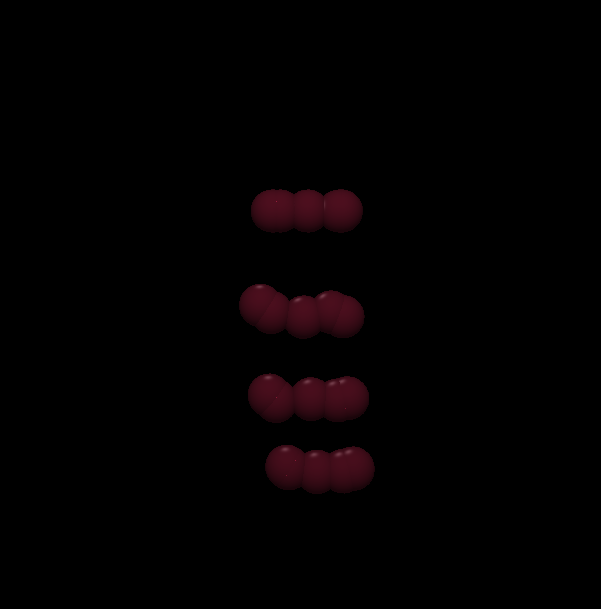
\includegraphics[scale=0.25]{check-in update}
\end{center}

The above image shows five strands of "hair" (currently just the hair nodes, but will be replaced by bezier curves).

\section{Additional References}
https://matthias-research.github.io/pages/publications/FTLHairFur.pdf


\end{document}

sys_open
readi()